\chapter{Contrucción de la aplicación}

El buscador semántico SAWA fue desarrollado en JavaEE\footnote{Java Platform, Enterprise Edition o Java EE
(anteriormente conocido como Java 2 Platform, Enterprise Edition o J2EE hasta la versión 1.4}
y liberado bajo licencia libre GPL3\footnote{\url{http://www.gnu.org/licenses/gpl.html}} el cual puede 
ser descargado del repositorio del portal github\footnote{\url{https://github.com/poldrosky/Sawa}} y
se puede mirar el funcionamiento en la página\footnote{\url{http://ingenieria.udenar.edu.co:8080/Sawa/}}. 

En la aplicación se usaron algoritmos  como lematizadores y similitud de palabras 
para hacer corrección ortográfica, en caso de que el usuario tenga error de digitación,
además de la construcción de un tesauro para que pueda hacer la búsqueda por sinónimos
de palabras.

Las siguientes son las características específicas del software construido:

\begin{itemize}
 \item Búsqueda General.
 \item Búsqueda por título.
 \item Búsqueda por autor.
 \item Auto completar palabras.
 \item Corrección de digitación.
 \item Búsqueda por sinónimos.
 \item Ordenamiento de resultados por mayor coincidencia.
\end{itemize}

En el diagrama de actividades de la Figura~\ref{figura:prueba1}  
se muestra como se realiza una búsqueda.

\begin{figure}[!ht]
\begin{center}
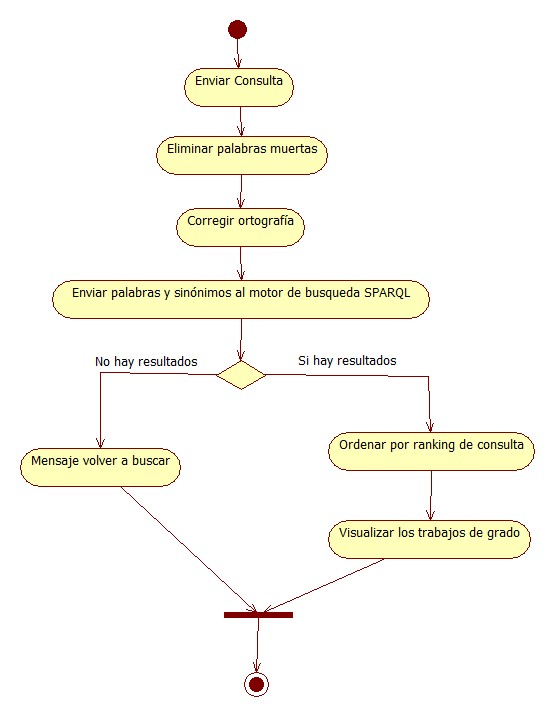
\includegraphics[width=10cm]{pictures/prueba1.jpg}
\end{center}
\caption{Diagrama de actividades de la búsqueda} \label{figura:prueba1}
\end{figure}


Para la construcción del software se tubo en cuenta la manera de 
realizar las consultas usando el lenguaje SPARQL y la extensión de 
postgresql pg\_similarity\footnote{\url{http://pgsimilarity.projects.pgfoundry.org}}.